\chapter{Results}
%In this chapter we expect you to list and explain all the results that you have achieved. Pictures can be useful to explain the results. Think about this chapter as something similar to the demo of the oral presentation. You can also include pictures about use-cases (you can also decide to add use cases to the high level overview chapter).
\begin{figure}[H]
\vspace{0.5cm}
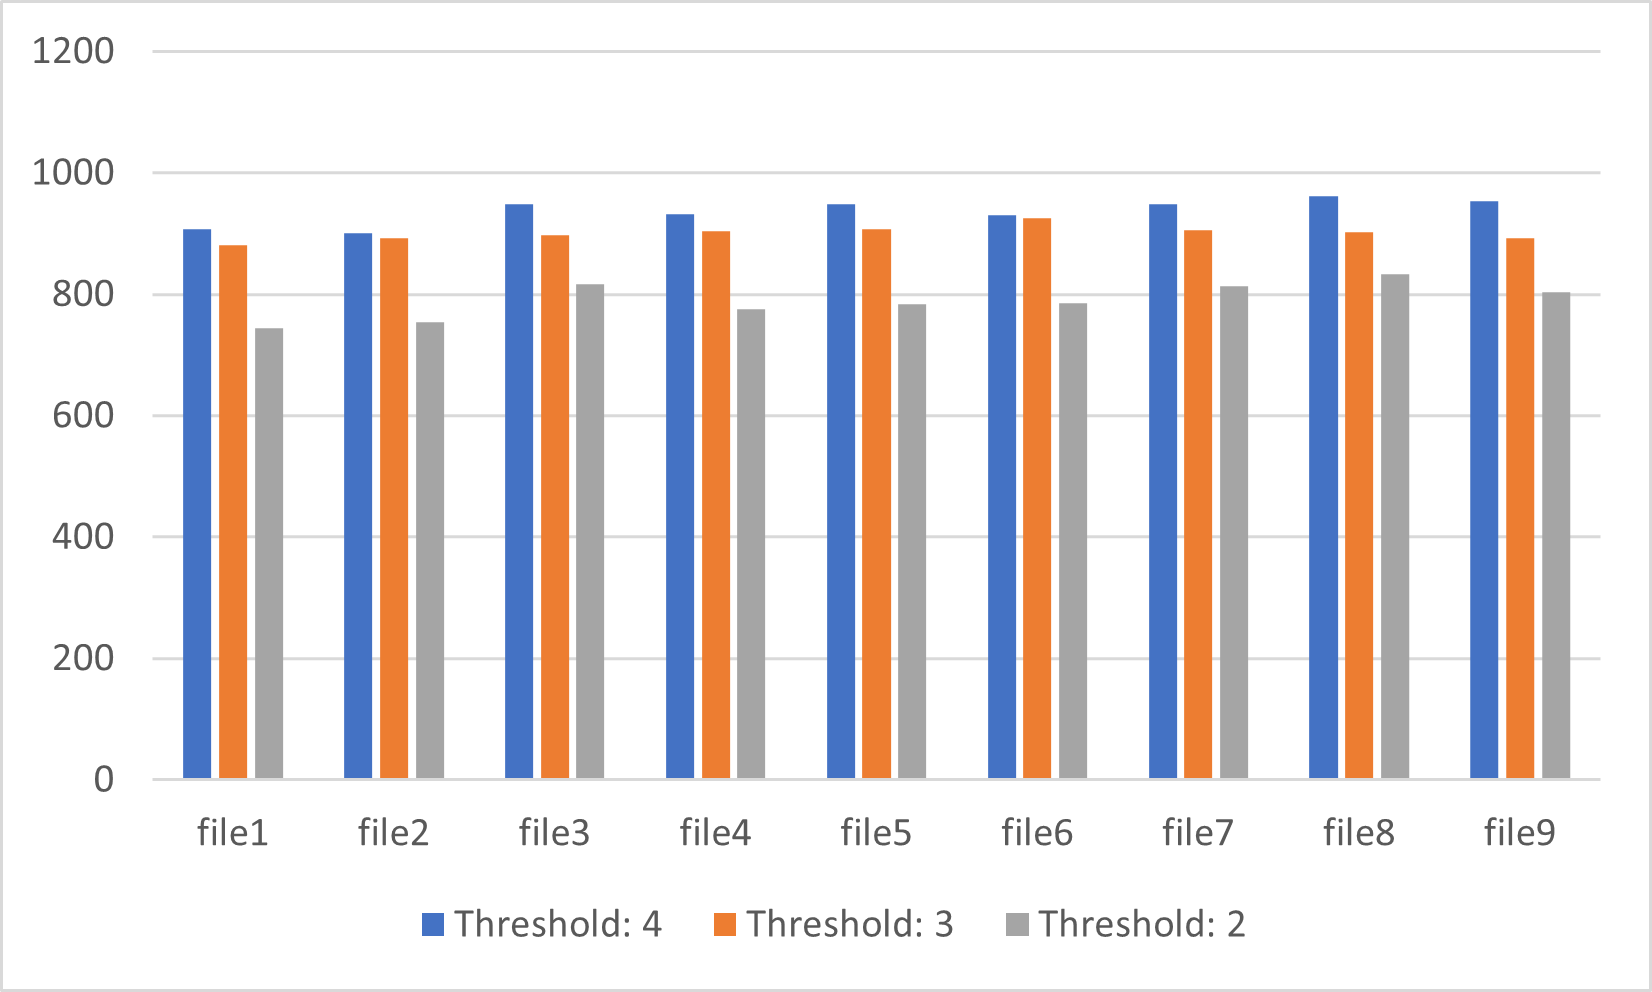
\includegraphics[width=\textwidth]{images/results.png}
\caption{results }
\label{fig:results} % This is the image label, with which you can refer to the image in any document location.
\end{figure}

----------
increasing the threshold it becomes easy to guess the correct response to use
decreasing the threshold few PUF are recognised as correct

find the best compromise
---------------


\section{Known Issues}
%If there is any known issue, limitation, error, problem, etc...explain it in this section. Use a specific subsection for each known issue. Issues can be related to many things, including design issues.
One of many issues of this implementation is that it is not secure from the Man-in-the-Middle attack, where a man can steal the challenge and response of the PUF.
There are some optimizations that can be done in order to avoid this kind of attack.


The main one is to eliminate a challenge-response once it is used; in this way it cannot be used in the future. This kind of implementation avoids replicant attacks.


Another type of security that can be used is encryption of the data, in order to ensure confidentiality in the communication. The encryption should be used, in particular, during the first communication between device and host, that means when the device sends all the challenge-response to the host.
It is important to say that the type of encryption and the necessity to encrypt or not depend on the type of device and by the level of sensibility of the datas that it can manage.


\section{Future Work}
Many are the implementations that can be done on this project, starting from the ones explained in the previous paragraph.


The main one could be to store the challenge-response in the file (host side) in the chipher way. In this way, if the file is stolen by an attacker he cannot be able to use the information.

Another one is to evaluate and store in a secure place the hash value of the file containing the challenge-response.
This kind of implementation can be used in order to ensure the integrity of the challenge-response of a particular device.
The idea consists in evaluating the hash value of the file before taking information from it and comparing it with the digest that we store in another place.
If the value is the same it means that the file is not corrupted.
%Adding a section about how to improve the project is not mandatory but it is useful to show that you actually understood the topics of the project and have ideas for improvements.



